
\section{Interface and explanation capability}

Elvira has a graphical user interface similar to other window
applications (see Figure~\ref{fig:prostanet}). It can operate in
three modes: edit, inference and learning. The \emph{edit mode} is
used to create and modify Bayesian networks and influence
diagrams. We do not describe it in detail because it is analogous
to other tools, such as Hugin, GeNIE or Netica. The differences
with some of these tools is that Elvira offers an undo-redo
facility, zoom and advanced features for modelling probabilities
by means of canonical models \cite{diez02x}. The \emph{learning
mode} is used to build Bayesian networks from databases, by
invoking the learning algorithms (see Sec.~\ref{sec:learning})
from the interface. In the rest of this section we describe in
detail the \emph{inference mode}, which has been enhanced by the
inclusion of advanced explanation facilities.
Figure~\ref{fig:prostanet} displays a screenshot of Elvira main
window in inference mode.

\begin{figure*}[hbt]
\begin{center}
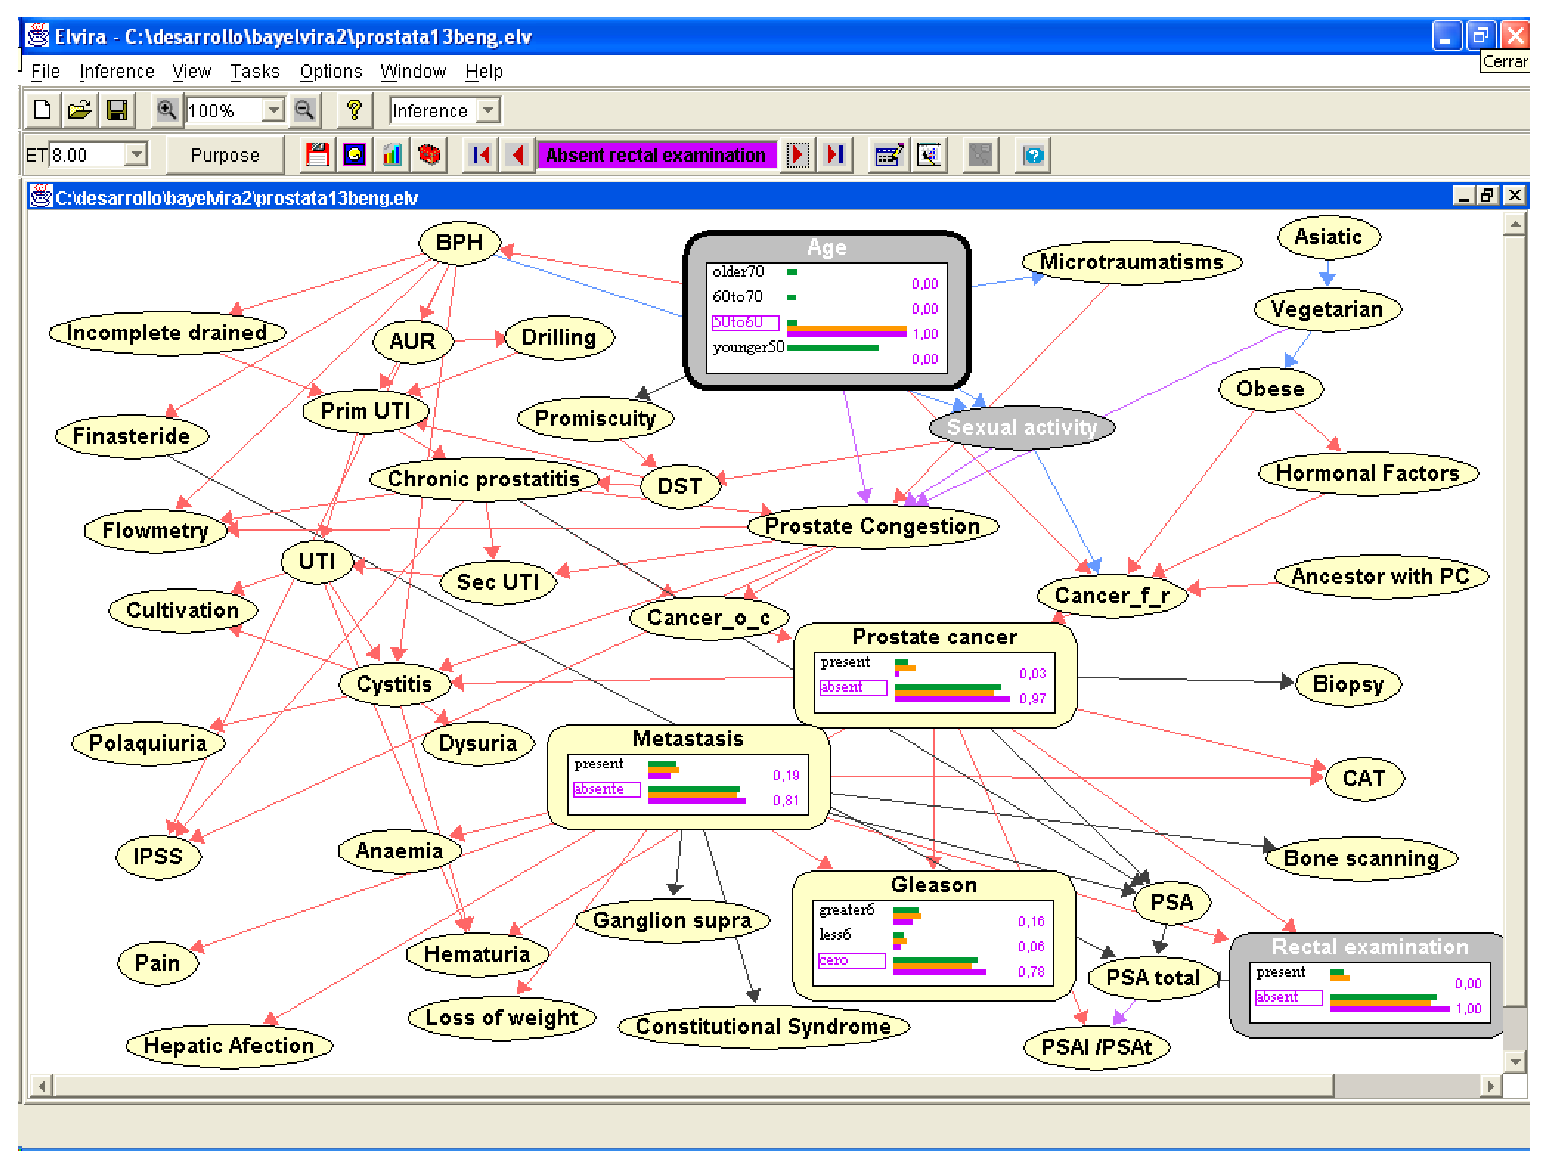
\includegraphics[width=155mm]{gui/fig/prostanet.eps}
\end{center}
\caption{Elvira main window in inference mode, displaying Prostanet,
a Bayesian network for the diagnosis in urology.}%
\label{fig:prostanet}%
\end{figure*}

Elvira offers several types of explanation: verbal and graphical, static and
dynamic, micro and macro---see \cite{lacave02a} for a detailed study of those
features and a review of explanation methods for Bayesian networks. Verbal
explanations are displayed by showing the information associated to given
nodes or links or, even, of the whole network. The verbal explanation of a
node selected by the user contains the following information: name, states,
parents and children, prior odds, posterior odds and other properties, such as
role and importance factor. The \emph{role} of a node is assigned by the
expert by classifying it into one of several categories, such as
\textit{symptom} or \textit{disease}. The \emph{importance factor}
is a value, between 0 and 10, assigned subjectively by the human
expert. The classification of nodes is used to generate verbal explanations,
such as ``\textsf{The disease \emph{[Name]} has the following RISK FACTORS:
\emph{[list of risk factors]}. It presents with the following SIGNS:
\emph{[list of signs]} and SYMPTOMS: \emph{[list of symptoms]}. There
are
several TESTS to confirm or discard its diagnosis:\emph{ [list of tests]}}''.

One of Elvira's explanation options, which distinguishes it from
other tools such as GeNie, Hugin or Netica, consists of
automatically colouring the links of the network, in order to
offer qualitative insight about the conditional probability
tables. The definition of the sign of an influence is very similar
to that used by Wellman \cite{wellman90a} in his qualitative
probabilistic networks (QPNs)---see also \cite{lacave02b}.

Another difference is that in Elvira, when switching from edit to
inference mode, the nodes whose importance factor is greater or
equal than the \emph{expansion threshold} (ET) are automatically
expanded. In Figure~\ref{fig:prostanet} the ET is set to 8.00.
Expanded nodes contain a line for each value/state, which displays
its name, a bar proportional to its probability and the numerical
value of its probability. In contrast to GeNie, Hugin or Netica,
Elvira has the ability to display several probability bars, one
for each \emph{evidence case} (an evidence case is a set of
findings). Additionally, the most probable value (for the current
case) is highlighted by a surrounding rectangle. The background
colour of observed nodes automatically changes to gray, so that
the user can easily identify the evidence of the current case.

Another difference between Elvira and other tools is its ability
to colour the nodes in order to show qualitatively the impact of
evidence. Again, this property is inspired in Wellman's work on
QPNs. However, the fact that our networks contain numerical
probabilities and that propagation of evidence is done by
quantitative algorithms allows us to determine the sign of
probability changes in many cases in which Wellman's algorithms
would lead to unknown signs.

Additionally, Elvira offers explanation facilities for each
evidence case, such as displaying the \emph{probability of
evidence}, performing a \emph{sensitivity analysis }(how the
evidence affects the posterior probabilities of a certain
hypothesis selected by the user) and, in contrast to other tools,
highlighting the \emph{chains of reasoning} followed in the
network from the evidence to the hypothesis---see \cite{lacave02b}
for further details.
